\section{Design Rationale: Educational use cases}

Since CodeInk targets instructors and students in CS education, we looked to two
main sources to guide its design: (1) lecture videos of instructors tracing
algorithms on blackboards, and (2) best practices from educational psychology.

\begin{figure}
\begin{center}
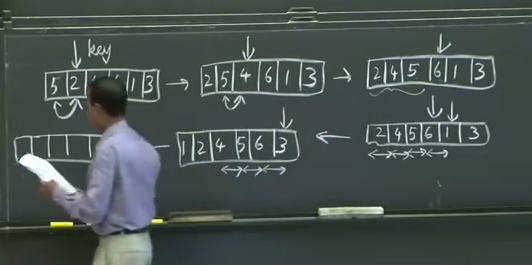
\includegraphics[width=0.7\columnwidth]{img/6006/insertion.png}
\end{center}
\caption{An instructor of MIT's introductory algorithms class draws a storyboard
to explain insertion sort on a concrete example of a list.}
\label{fig:6006-insertion}
\end{figure}


\subsection{Concrete traces}
We observed that instructors explain algorithms by drawing concrete examples of
data structures - for example, a specific list when explaining insertion sort
(\fig{fig:6006-insertion}) - and then trace the algorithm's behavior on that
example. We call this a \emph{concrete trace}, because the instructor does not
explain the algorithm in general or graphically draw flow control. Instead, they
unfold the loops and branches of an algorithm's pseudocode into a sequence of
concrete steps.
% This approach is in line with findings that students need to see multiple
% examples of an algorithm's behavior to build their
% understanding~\cite{Vainio2007}.
CodeInk targets the task of tracing algorithms through concrete examples, rather
than explaining them in the abstract.

%Also, according to cognitive load theory, novices can learn better by watching
%experts solve problems that would be too difficult for novices to solve on
%% their own~\cite{Linn1992, Sweller1985}. The instructor's worked examples give
%% students
%an opportunity to get the gist of an algorithm, before they attempt to trace it
%on their own. 

\subsection{Level of abstraction}
The instructor's explanation occurs at a high level of graphical abstraction.
They rarely write language-specific code on the board (e.g. in Python), and will
instead opt for a combination of pseudocode and data structure diagrams. This is
because the pseudocode and diagrams abstract away language-specific details that
are not essential to understanding the strategy behind the algorithm. CodeInk
focuses on enabling tracing by direct manipulation of data structure diagrams.
% This should not be confused with the previous point: the traced steps are
% concrete, and do not include control abstraction (e.g. loops).


\begin{figure}
\begin{center}
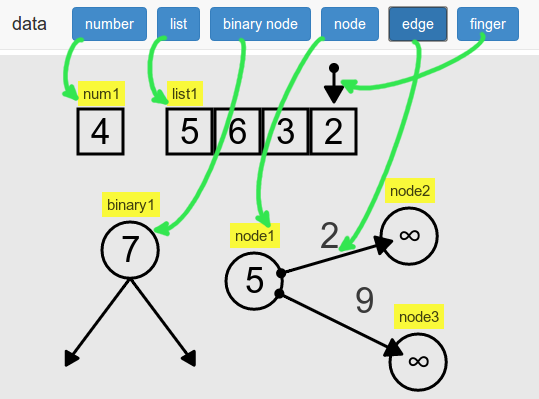
\includegraphics[width=0.8\columnwidth]{img/visual-vocabulary.png}
\end{center}

\caption{CodeInk's visual vocabulary and Data Palette. The green arrows are for
illustration only, and show how data structures (numbers, lists, binary tree
nodes, graph nodes, edges) and fingers can be dragged onto the stage to
setup an example.}
\label{fig:visual_vocab}
\end{figure}

\subsection{Visual vocabulary}
When drawing data structures, instructors use a familiar, consistent visual
vocabulary: lists are drawn as a row of boxes (\fig{fig:6006-insertion}), and
trees and graphs are drawn as circles connected by arrows. To represent values,
each object has a number inscribed within or adjacent to it; all examples in
lecture videos we watched were numerical. We designed CodeInk's visual
vocabulary (\fig{fig:visual_vocab}) to mirror these conventions.

\begin{comment}
Instructors add to this vocabulary using arrows and colors. Arrows are
interchangably used to show transitions between storyboard frames, or to point
to the current focus of the algorithm (\fig{fig:6006-insertion}). The former is
an artifact of the need to draw snapshots when using blackboards, while the
latter is an important visual cue for following the algorithm's progress. Colors
are also used to visualize state; for example, to mark graph nodes as visited,
they are filled with a different color. CodeInk's visual vocabulary includes
\emph{fingers}, which can be attached to any on-screen object, and a \emph{fill}
gesture (explained later) that can be used to color a data structure.
\end{comment}

\subsection{Student traces and targeted feedback}
In a multi-national study, Lister et. al~\cite{Lister2004} found that tracing
code is a prerequisite skill for problem solving and the ability to write
programs. They further stated that programming courses should ``first teach
systematic tracing as a base skill, then allow students to build [\ldots] upon
that''.
% found that students in introductory programming courses could not consistently
% demonstrate an understanding of code by manually tracing it. The researchers
% noted that ``even when our principal aim is to teach students to write code,
% we require students to learn by reading code''
In addition to being an authoring tool for instructors, we believe CodeInk
enables students to practice tracing pseudocode on examples. The student has the
freedom to explore an algorithm's behavior, perhaps making mistakes along the
way. As a basis for targeted feedback~\cite{Balzer1989}, CodeInk records the
student's effort, so a teacher can analyze both the final answer, and the
process by which it was reached.
% Show your work

%Finally, students eventually need to learn to write algorithms in a real
%programming language. CodeInk provides a mapping from visual data
%structure changes to lines of Python code. This serves as a form of
%instructional scaffolding~\cite{Pea2004} to help students acquire
%basic programming skills.

\begin{comment}

CodeInk supports three main educational use cases:

\begin{itemize}\itemsep0pt

\item Instructors can easily create algorithm explanations that can be
used in a live class or disseminated online.

\item Students can step through instructor-created explanations to learn
both the algorithms and basic Python constructs, such as list
manipulation operators.

\item Students can solidify their understanding by tracing an algorithm
on new input data. CodeInk records all user interactions, which enables
instructors to give targeted feedback~\cite{Balzer1989} on the student's
problem-solving process.

\end{itemize}

\end{comment}

